\section{Results}

\begin{frame}[c,fragile,allowframebreaks]{Accuracy Overview}
    \pause
    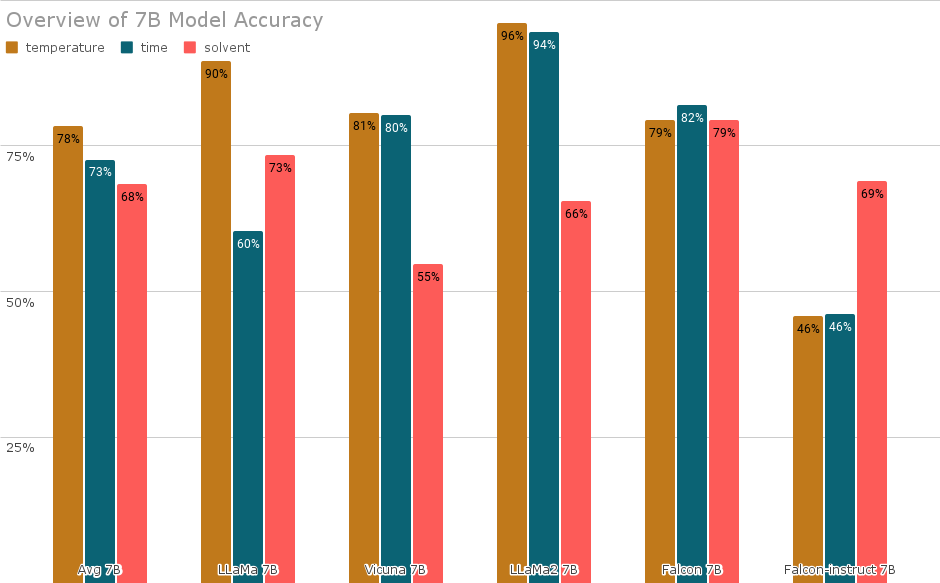
\includegraphics[height=0.7\textheight]{overview_7b_accuracy}
    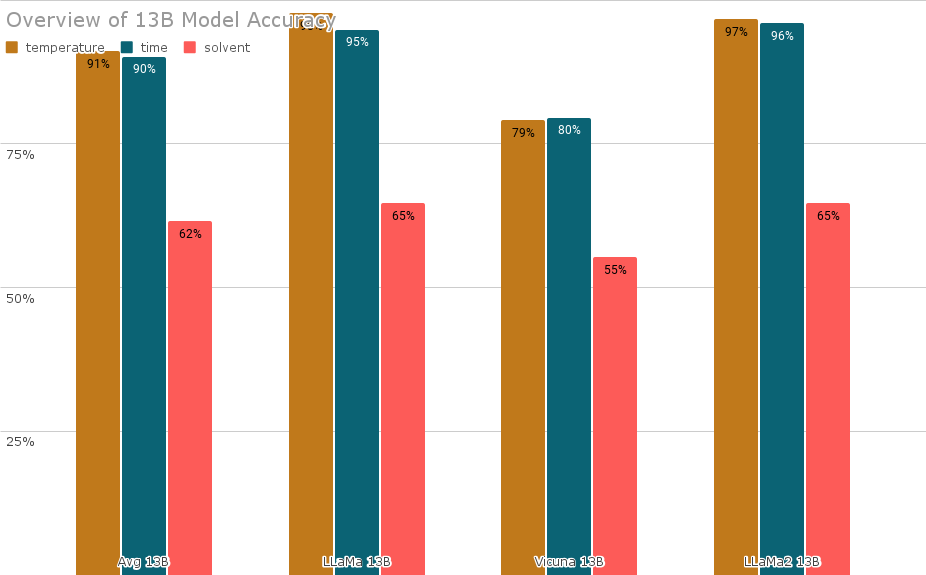
\includegraphics[height=0.7\textheight]{overview_13b_accuracy}
    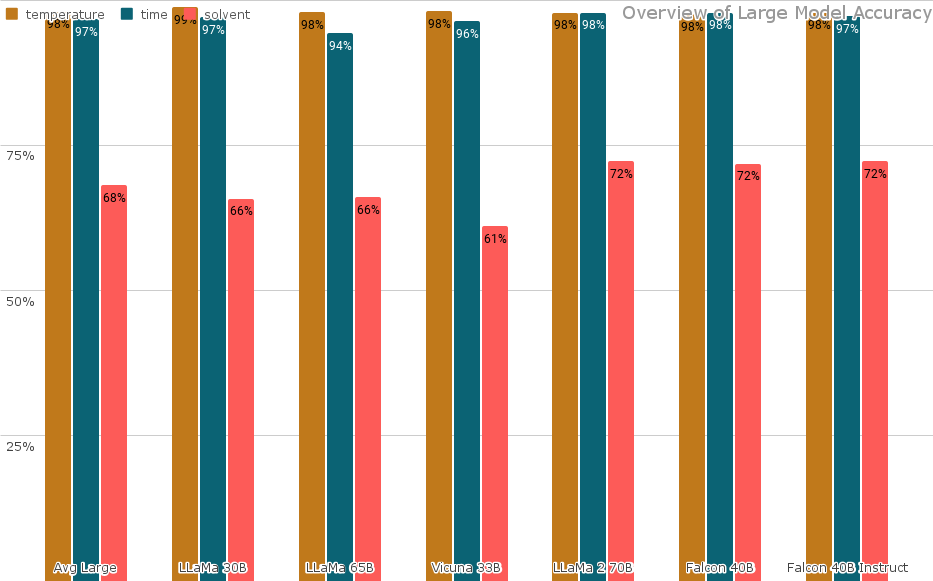
\includegraphics[height=0.7\textheight]{overview_large_accuracy}
\end{frame}



\begin{frame}<handout>[c]{Note on Interesting Outliers}
    \begin{columns}
        \column{0.3\textwidth}
    7B
    \begin{itemize}
        \item \gls{llama}-7B accuracy on \ttemp and \ttime vary substantially across models, but are mostly similar within one model
        \item \tsolv accuracy of \gls{vicuna} bad somehow
        \item Bad \ttemp and \ttime accuracy of \gls{falcon}-instruct
        \item Decent performance from \gls{llama2} overall
    \end{itemize}
        \column{0.3\textwidth}
        \large
        13B
        \begin{itemize}
            \item \gls{vicuna} still lagging behind, though while \gls{falcon} does not have a 13B variant, it should still be worse
            \item Accuracy on \tsolv seems to have gotten worse, on average and for individual models
        \end{itemize}
        \column{0.3\textwidth}
        \large
        30B+
        \begin{itemize}
            \item Average Accuracy very high
            \item \tsolv accuracy only 72\% though, that was higher in 7B models!
        \end{itemize}
    \end{columns}
\end{frame}

\subsection{Frequent Mistakes}

\begin{frame}[c,fragile,allowframebreaks]{Unit Confusion}
    \pause
    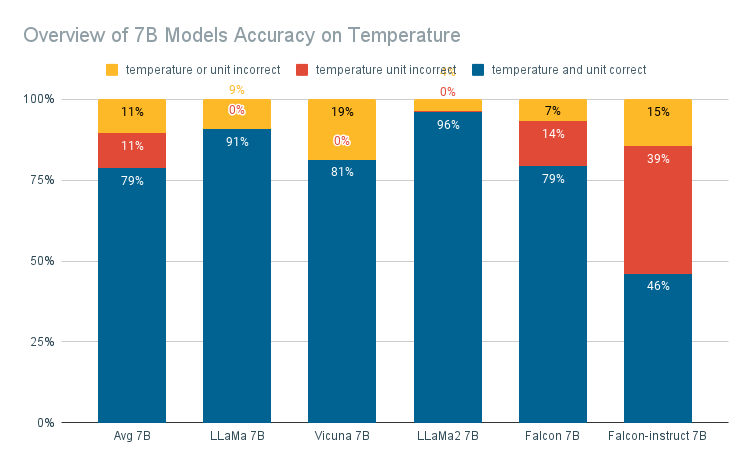
\includegraphics[height=0.7\textheight]{overview_7b_temp}
    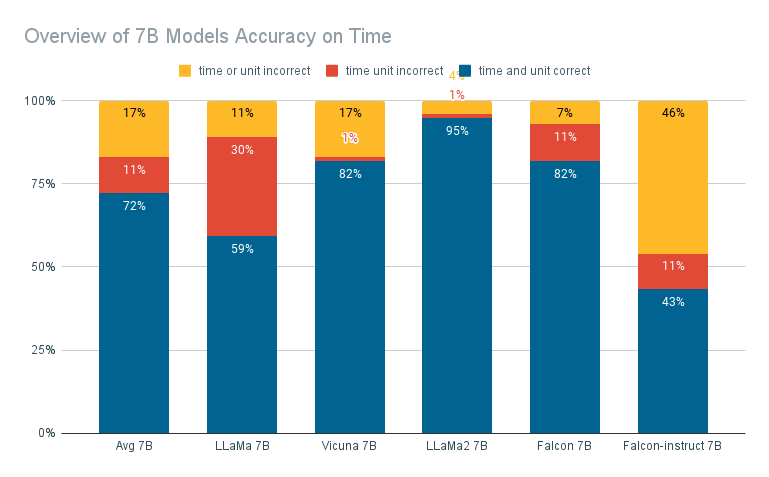
\includegraphics[height=0.7\textheight]{overview_7b_time}
    % \begin{columns}
    %     \column{0.35\textwidth}
    % 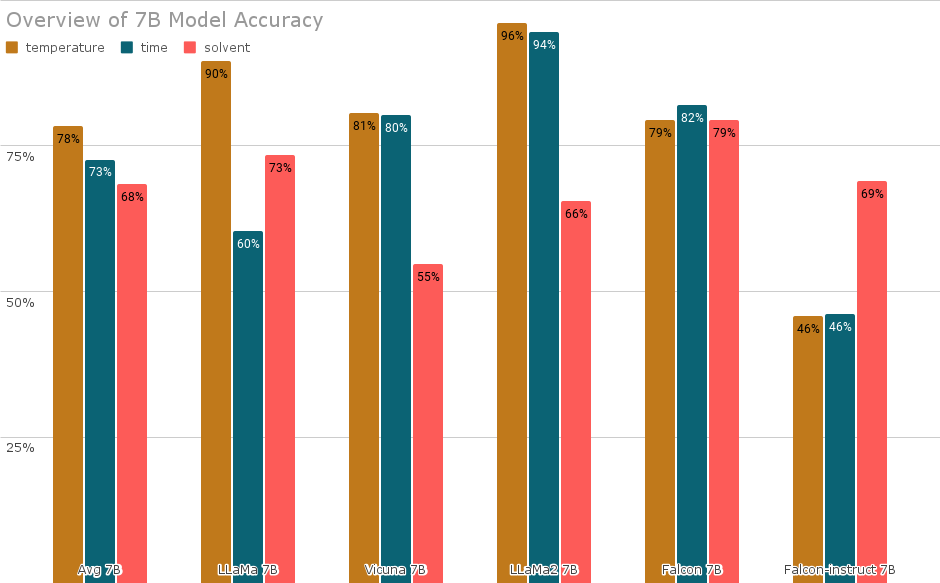
\includegraphics[width=\textwidth]{overview_7b_accuracy}
    % \column{0.65\textwidth}
    % 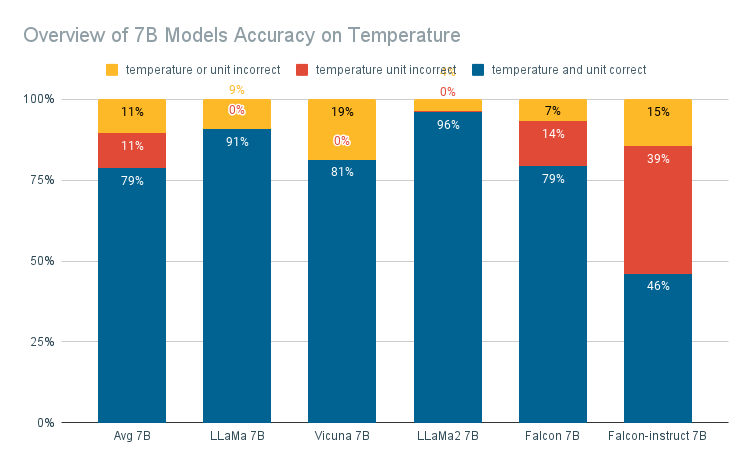
\includegraphics[height=0.7\textheight]{overview_7b_temp}
    % \end{columns}
    % \newpage
    % \begin{columns}
    %     \column{0.35\textwidth}
    % 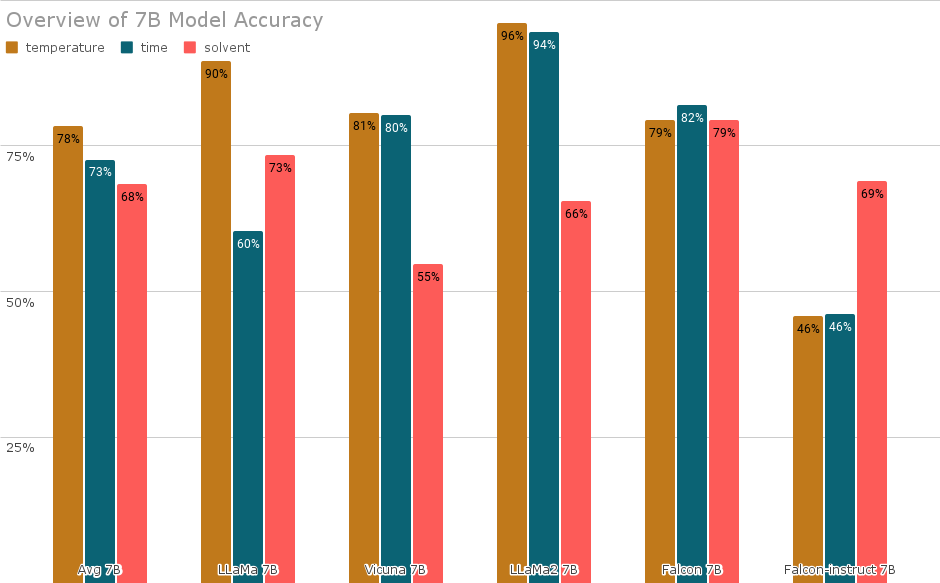
\includegraphics[width=\textwidth]{overview_7b_accuracy}
    % \column{0.65\textwidth}
    % 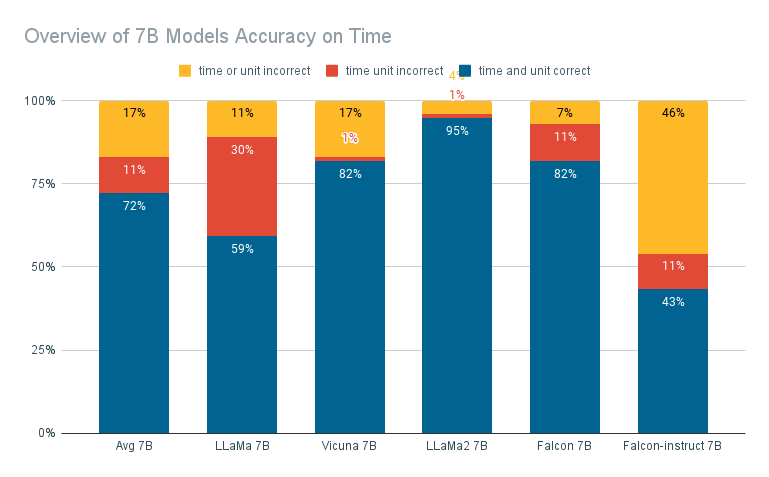
\includegraphics[height=0.7\textheight]{overview_7b_time}
    % \end{columns}
\end{frame}

\begin{frame}<handout>[c]{Note on Unit Confusion}
    \Large 
    \begin{itemize}
        \item Does happen in fewer than 0.5\% (0-4 cases) for models sized 13B or more
    \end{itemize}
\end{frame}

\begin{frame}[c,fragile,allowframebreaks]{Solvent Resolution}
    \centering
    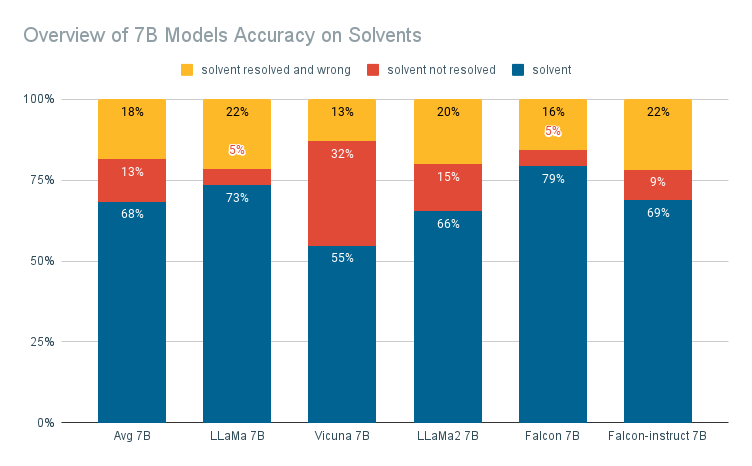
\includegraphics[height=0.7\textheight]{overview_7b_solv}
    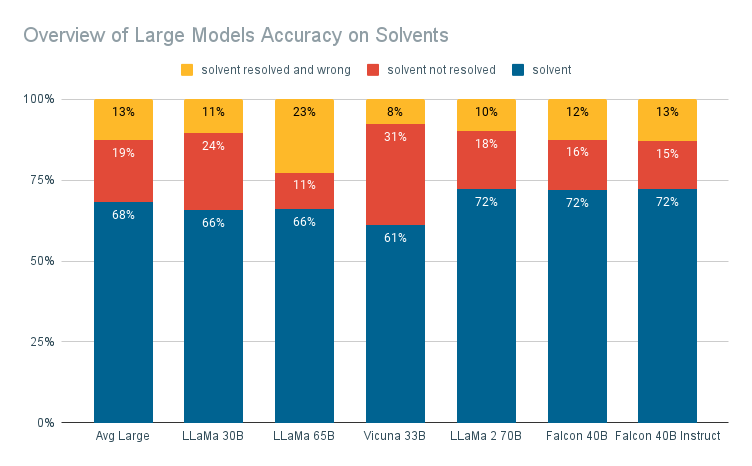
\includegraphics[height=0.7\textheight]{overview_large_solv}
\end{frame}


\begin{frame}[c]{Solvent Resolution?}
    \large
    One hypothesis: Models \textit{are} getting more accurate, but there is a failure in resolving the compounds.

    \vspace{2em}
    \pause

    Remember `distilled H2O'?

    \vspace{2em}
    \pause

    This may be true in particular for the \tsolv \texttt{N,N-DIMETHYLACETAMIDE} (\texttt{cid} 31374), where the synthesis paragraphs contain none of its 125 synonyms in 34 cases (or about 4.37\% of the dataset). 
\end{frame}

\begin{frame}[c]{Fine-Tuning: Excerpt 1}
    \code{input.py}{input}{Excerpt of what could be found in a custom dataloader. \mpy{text} describes any string the model may be provided as input. The tokenizer converts any string to a list of tokens and an attention mask, among other things.\\
    Similar code can be found in tutorials and official sources, e.g. \gls{microsoft} \cite{deepspeedexamples_2023}
}
\end{frame}


\begin{frame}[c]{Fine-Tuning: Failure 1}
    \code{output2.py}{output2}{A model fine-tuned like this returns the following. The \mpy{"} where actually inserted during conversion to \texttt{json} from \texttt{jsonformer}.}
    \only<handout>{
        \large
        Fundamentally, no idea what is going on. It works for others, and it could still be one of many different things that actuatlly happened.
    }
\end{frame}


\begin{frame}[c]{Fine-Tuning: Excerpt 2} 
    \large
    \begin{itemize}[<+(1)->]
        \item Using the \gls{hf} \texttt{trl} (Transformer Reinforcement Learning) library
        \item \mpy{DataCollator} are used for batch-processing inputs
        \item \mpy{DataCollatorForLanguageModeling} abstracting away tokenization, uses \mpy{"text"}-key for training in other examples
        \item Specifically, the example uses \mpy{DataCollatorForCompletionOnlyLM}, deriving from it
    \end{itemize}
\end{frame}


\begin{frame}[c]{Fine-Tuning: Failure 2}
    \code{error.py}{error}{Error when providing \mpy{DataCollatorForCompletionOnlyLM} with a dataloader similar to those in examples.\\Counterintuitively, this is not a \mpy{KeyError}.}
    It also fails when manually tokenizing before the \mpy{DataCollator} (providing tokenized \mpy{"input_ids"} etc. as key, using this or a different \mpy{DataCollator}).
\end{frame}
